\documentclass[10pt, spanish, pdftex]{../.template/template}	

%%%%%%%%%%%%%%%%%%%%%%%%%%%%%%%%%%%%%%%%%%%%%%%%%%%%%%%%
%               UC3M Work report template              %
%           Universidad Carlos III de Madrid           %
%              Author: Aitor Alonso Núñez              %
%              Last update: March 8, 2018              %
%%%%%%%%%%%%%%%%%%%%%%%%%%%%%%%%%%%%%%%%%%%%%%%%%%%%%%%%

%%%%% Preamble %%%%%
\usepackage{fancyhdr}				% To add header and footer
\usepackage{graphicx}				% To add images
\usepackage{caption}				% To add captions
\usepackage{subcaption}				% To add subcaptions
\usepackage{lipsum}					% Example Lorem ipsum text
\usepackage[hidelinks]{hyperref}	% Index elements works as cross references. Also functional links to internet pages
\usepackage{nameref}				% Allow to add labels with \label{name} which can be reference with \nameref{name}
\author{Aitor Alonso Núñez}			% This is me!

\usepackage{listings}
\graphicspath{{images/}}

\newcommand*{\namerefs}[1]{\textit{\underline{\color{uc3mNewBlue}\nameref{#1}}}}

%%%%% Coauthors info %%%%%
%%[1-2] If you want to show coauthors email address on the title page, enable \emailtrue. Otherwise, enable \emailfalse
\emailtrue
% \emailfalse
%% If coauthors are between 1 and 2 uncomment these options. Comment it otherwise.
%% You can leave empty keys {} if you need to.
\coauthorstwotrue		% coauthors two = true
\coauthorsthreefalse	% coauthors three = false
\coauthorsfourfalse		% coauthors four = false
\coauthorstwo{Aitor Alonso Núñez}{NIA 100346169}{Gr. 83}{Daniel Gak Anagrov}{NIA 100318133}{Gr. 83}
%%[3] If you enabled \emailtrue, uncomment the option below
\emailstwo{100346169@alumnos.uc3m.es}{100318133@alumnos.uc3m.es}

%% If coauthors are between 1 and 2 uncomment these options. Comment it otherwise.
%% You can leave empty keys {} if you need to.
% \coauthorstwofalse		% coauthors two = false
% \coauthorsthreetrue		% coauthors three = true
% \coauthorsfourfalse		% coauthors four = false
% \coauthorsthree{Name1 Lastname1}{NIA 100XXXXXX}{Gr. XX}{Name2 Lastname2}{NIA 100XXXXXX}{Gr. XX}{Name3 Lastname3}{NIA 100XXXXXX}{Gr. XX}
%% If you want to show on the title page the email address of these coauthors uncomment the next options
%% and comment \emailfalse. In other case, comment everything except \emailfalse
% \emailsthree{email1@domain.tld}{email2@domain.tld}{email3@domain.tld}

%%[4] If coauthors are between 1 and 2 uncomment these options. Comment it otherwise.
%% You can leave empty keys {} if you need to.
% \coauthorstwofalse		% coauthors two = false
% \coauthorsthreefalse		% coauthors three = false
% \coauthorsfourtrue		% coauthors four = true
% \coauthorsfour{Name1 Lastname1}{NIA 100XXXXXX}{Name2 Lastname2}{NIA 100XXXXXX}{Name3 Lastname3}{NIA 100XXXXXX}{Name4 Lastname4}{NIA 100XXXXXX}
%% If you want to show on the title page the email address of these coauthors uncomment the next options
%% and comment \emailfalse. In other case, comment everything except \emailfalse
% \emailsfour{email1@domain.tld}{email2@domain.tld}{email3@domain.tld}{email4@domain.tld}


%%%%% Basic data about the document (Degree, subject, title, campus, page number custom text) %%%%%
\documentdata{Grado en Ingeniería Informática}{Aprendizaje Automático}{Práctica 2:\\Aprendizaje basado en instancias}{Página }

%%%%% Page style %%%%%
\header
\footer
\pagestyle{fancy}
\begin{document}

%%%%% Page title %%%%%
\titleMain

%%%%% Index %%%%%
\tableofcontents 	% We add the index
\newpage 			% And before index we start on a new page

%%%%% CONTENIDO DEL DOCUMENTO %%%%%
%% VERY IMPORTANT!!! On the first line of this .tex file, select Spanish or English language to coincide with document text language
\section{Introducción}
    \p{Este documento sirve como memoria de la práctica 2: \textit{Aprendizaje basado en instancias}, de la asignatura Aprendizaje
    Automático. En la misma, hemos tenido que programar un agente basado en instancias, esto es, que aprenda a jugar al Mario mediante
    comparación y evaluación del momento del juego actual contra momentos almacenados en una base de conocimiento.}
    \p{A lo largo del presente documento se describirá el \namerefs{td}, donde comentamos todo lo referente a la toma de ejemplos y
    carga inicial de la base de conocimiento; \namerefs{f}, donde se describen y detallan las funciones utilizadas para clasificar y
    evaluar instancias; y por último, una \namerefs{e}, \namerefs{c} y \namerefs{cp}}

\section{Tratamiento de datos}\label{td}
    \subsection{Toma de ejemplos}\label{tde}
    % Explicar que solo hemos tomado ejemplos del agente humano P2. Y que, como las instancias en las que mario tira una bola de fuego nos
    % perjudica porque el efecto de reward tiene lugar varios ticks adelante en el futuro, se ha eliminado la posibilidad de tomar este
    % tipo de acciones. Para ello, se ha eliminado del código del agente humano la posbilidad de pulsar la tecla speed, luego aunque el
    % agente humano pulse la tecla speed, mario no dispra.
    \p{Para la toma de ejemplos hemos utilizado únicamente el agente humano \texttt{P2HumanAgent}, ya que consideramos que
    el agente a programar aprende por imitación, mediante comparación y evaluación de las instancias, por lo que una toma de
    ejemplos de un comportamiento humano sería bastante adecuada por los siguientes motivos.}
    \p{El comportamiento humano, en este contexto, realiza acciones con sentido. Esto es así puesto que somos personas que
    sabemos jugar al Mario, conocemos los objetivos a puntuar en esta práctica (acabar el nivel con la mayor recompensa), y
    realizamos las acciones necesarias en cada instante del juego para lograr tal fin.}
    \p{Si bien el comportamiento humano tiene cierto grado de aleatoriedad, puesto que no efectúa la misma acción de la misma manera
    en dos situaciones idénticas (ya sea por tiempo de reacción del agente humano, estrategias a largo plazo, etc.), en general la
    acción realizada tiene sentido, es correcta, y va enfocada a conseguir el objetivo final anteriormente descrito.}
    \p{Luego, puesto que nuestro agente inteligente a programar aísla cada instancia de cada momento del juego, y la analiza en
    base a valores objetivos (sin contexto anterior o futuro), consideramos que elimina la aleatoriedad humana del aprendizaje,
    quedándose solo con lo importante (situación $>$ acción $>$ evaluación).}

        \subsubsection{Estrategia de selección de instancias}\label{esi}
        \p{Puesto que posteriormente en nuestro agente vamos a evaluar las instancias de nuestra base de conocimiento en base a la
        recompensa futura que se consiguió realizando la acción relacionada con cada instancia, conviene evitar instancias de
        entrenamiento (que acabarán posteriormente en la base de conocimiento) que contengan acciones que proporcionaron recompensa
        muy a futuro, ya que podría meter ruido y dificultar la evaluación.}
        \p{Un ejemplo de este tipo de acciones es la de disparar con Mario. Desde que Mario dispara una bola de fuego, pueden pasar
        varios segundo de juego hasta que un enemigo es eliminado, y por tanto hasta que se consigue la recompensa por ello. Puesto
        que un segundo de juego son 24 ticks, y vamos a evaluar las instancias en base a la recompensa que conseguimos en torno a
        6 -- 24 ticks después de realizar la acción correspondiente, es mejor ignorar estas situaciones.}
        \p{Para directamente evitar este tipo de instancias a la hora de la toma de ejemplos, hemos desactivado en nuestro agente
        humano \texttt{P2HumanAgent} la posibilidad de pulsar la tecla ``S'', correspondiente con disparar y correr. Así, aunque
        el jugador presione la tecla ``S'', el agente no está capturando el evento, pues hemos eliminado el código correspondiente
        a dicha tecla de la función \texttt{getAction()}.}
    
    \subsection{Atributos}\label{a} % Descripción y rango de valores
    \p{Nuestras instancias de entrenamiento, que han sido tomadas con el agente humano \texttt{P2HumanAgent} con ayuda del
    código de toma de datos contenido en el fichero \texttt{tools/TrainingFile.java}, consta de los siguientes atributos en
    este orden, si bien no todos son utilizados posteriormente en el agente bot inteligente, producto de esta práctica.}
    \subsubsection{Atributos para ayudar a localizar o identificar la instancia de entrenamiento}
    \begin{enumerate}
        \item \textbf{timeSpent:} Tiempo gastado en segundos del juego (\texttt{short})
        \item \textbf{timeLeft:} Tiempo restante en segundos del juego (\texttt{short})
    \end{enumerate}
    \subsubsection{Atributos relacionados con la intermediateReward}
    \begin{enumerate}
        \setcounter{enumi}{2}
        \item \textbf{intermediateReward:} Recompensa actual en el momento de la instancia (\texttt{short})
        \item \textbf{intermediateRewardWonLastTick:} Recompensa obtenida respecto al tick anterior (1/24s) (\texttt{short})
        \item \textbf{intermediateRewardWonLast6Ticks:} Recompensa obtenida respecto a los 6 ticks anteriores (1/4s) (\texttt{short})
        \item \textbf{intermediaRewardWonFuture6Ticks:} Recompensa obtenida 6 ticks después (1/4s) de ejecutar la acción de esta instancia (\texttt{short})
        \item \textbf{intermediaRewardWonFuture12Ticks:} Recompensa obtenida 12 ticks después (1/2s) de ejecutar la acción de esta instancia (\texttt{short})
        \item \textbf{intermediaRewardWonFuture24Ticks:} Recompensa obtenida 24 ticks después (1s) de ejecutar la acción de esta instancia (\texttt{short})
    \end{enumerate}
    \subsubsection{Atributos relacionados con la matriz de observación (mergeObs)}
    \begin{enumerate}
        \setcounter{enumi}{8}
        \item \textbf{nearestEnemyLeftDistance:} Distancia euclídea al enemigo más cercano a la izquierda de Mario (\texttt{float})
        \item \textbf{nearestEnemyLeft\_X:} posición X de la mergeObs del enemigo más cercano por la izquierda (\texttt{byte})
        \item \textbf{nearestEnemyLeft\_Y:} posición Y de la mergeObs del enemigo más cercano por la izquierda (\texttt{byte})
        \item \textbf{nearestEnemyRightDistance:} Distancia euclídea al enemigo más cercano a la derecha de Mario (\texttt{float})
        \item \textbf{nearestEnemyRight\_X:} posición X de la mergeObs del enemigo más cercano por la derecha (\texttt{byte})
        \item \textbf{nearestEnemyRight\_Y:} posición Y de la mergeObs del enemigo más cercano por la derecha (\texttt{byte})
        \item \textbf{nearestBlockLeftDistance:} Distancia euclídea al bloque más cercano a la izquierda de Mario (\texttt{float})
        \item \textbf{nearestBlockLeft\_X:} posición X de la mergeObs del bloque más cercano por la izquierda (\texttt{byte})
        \item \textbf{nearestBlockLeft\_Y:} posición Y de la mergeObs del bloque más cercano por la izquierda (\texttt{byte})
        \item \textbf{nearestBlockRightDistance:} Distancia euclídea al bloque más cercano a la derecha de Mario (\texttt{float})
        \item \textbf{nearestBlockRight\_X:} posición X de la mergeObs del bloque más cercano por la derecha (\texttt{byte})
        \item \textbf{nearestBlockRight\_Y:} posición Y de la mergeObs del bloque más cercano por la derecha (\texttt{byte})
        \item \textbf{nearestCoinLeftDistance:} Distancia euclídea a la moneda más cercana a la izquierda de Mario (\texttt{float})
        \item \textbf{nearestCoinLeft\_X:} posición X de la mergeObs de la moneda más cercana por la izquierda (\texttt{byte})
        \item \textbf{nearestCoinLeft\_Y:} posición Y de la mergeObs de la moneda más cercana por la izquierda (\texttt{byte})
        \item \textbf{nearestCoinRightDistance:} Distancia euclídea a la moneda más cercana a la derecha de Mario (\texttt{float})
        \item \textbf{nearestCoinRight\_X:} posición X de la mergeObs de la moneda más cercana por la derecha (\texttt{byte})
        \item \textbf{nearestCoinRight\_Y:} posición Y de la mergeObs de la moneda más cercana por la derecha (\texttt{byte})
        \item \textbf{numEnemiesObserved:} número total de enemigos identificados en la matriz de observación (\texttt{short})
        \item \textbf{numCoinsObserved:} número total de monedas identificadas en la matriz de observación (\texttt{short})
    \end{enumerate}
    \subsubsection{Atributos booleanos o binarios}
    \begin{enumerate}
        \setcounter{enumi}{28}
        \item \textbf{enemyNearRight:} valor numérico binario (0-1) que indica si hay (1) o no (0) enemigos en una submatriz de la matriz de observación ([fil][col] == [8-9][10-11]) (\texttt{byte})
        \item \textbf{blockNearRight:} valor numérico binario (0-1) que indica si hay (1) o no (0) obstáculos en una submatriz de la matriz de observación ([fil][col] == [8-9][10-11]) (\texttt{byte})
        \item \textbf{enemyAheadOnFloorHeight:} valor numérico binario (0-1) que indica si hay (1) o no (0) enemigos en una submatriz de la matriz de observación ([fil][col] == [10][10-11]) (\texttt{byte})
        \item \textbf{blockAheadOnFloorHeight:} valor numérico binario (0-1) que indica si hay (1) o no (0) obstáculos en una submatriz de la matriz de observación ([fil][col] == [10][10-11]) (\texttt{byte})
        \item \textbf{abyssAhead:} valor numérico binario (0-1) que indica si hay (1) o no (0) foso/abismo/acantilado delante (en columna [10]) (\texttt{byte})
        \item \textbf{isMarioOnGround:} valor numérico binario (0-1) que indica si Mario está (1) o no está (0) en el suelo (\texttt{byte})
        \item \textbf{isMarioAbleToJump:} valor numérico binario (0-1) que indica si Mario puede (1) o no puede (0) saltar (bloqueo de salto) (\texttt{byte})
        \item \textbf{isMarioAbleToShoot:} valor numérico binario (0-1) que indica si Mario puede (1) o no puede (0) disparar (\texttt{byte})
        \item \textbf{isMarioCarrying:} valor numérico binario (0-1) que indica si Mario está (1) o no está (0) llevando un caparazón (\texttt{byte})
        \item \textbf{enemyWasKilledBin:} valor numérico binario (0-1) que indica si Mario si (1) o no (0) ha muerto un enemigo en la instancia actual (\texttt{byte})
        \item \textbf{marioWasInjuredBin:} valor numérico binario (0-1) que indica si Mario si (1) o no (0) ha ha sido herido Mario en la instancia actual (\texttt{byte})
        \item \textbf{isSlopeDown:} valor numérico binario (0-1) que indica si hay (1) o no (0) un foso/abismo/acantilado delante (en matriz de observación [16][10] no hay bloque) (\texttt{byte})
    \end{enumerate}
    \subsubsection{Otros atributos}
    \begin{enumerate}
        \setcounter{enumi}{40}
        \item \textbf{coinsGainedLastTick:} número de monedas conseguidas respecto al tick anterior (\texttt{byte})
        \item \textbf{marioMode:} modo actual de Mario: 0,1,2 == pequeño, grande, fuego (\texttt{byte})
        \item \textbf{marioStatus:} estado actual de Mario: 0,1,2 == muerto/derrota, victoria, corriendo/jugando (\texttt{byte})
        \item \textbf{actionKey:} acción o acciones realizadas durante esta instancia, codificada como un valor numérico que diferencia varias situaciones (\texttt{byte})
        \begin{itemize}
            \item Ninguna acción o tecla pulsada: \textbf{0}
            \item Salto (tecla A): \textbf{1}
            \item Derecha (tecla flecha derecha): \textbf{2}
            \item Derecha-salto (teclas flecha derecha + A): \textbf{3}
            \item Derecha-disparar (teclas flecha derecha + S): \textbf{4} (no puede existir en esta toma de ejemplos)
            \item Derecha-salto-disparar (teclas flecha derecha + A + S): \textbf{5} (no puede existir en esta toma de ejemplos)
            \item Izquierda (tecla flecha izquierda): \textbf{6}
            \item Izquierda-salto (teclas flecha izquierda + A): \textbf{7}
            \item Izquierda-disparar (teclas flecha izquierda + S): \textbf{8} (no puede existir en esta toma de ejemplos)
            \item Izquierda-salto-disparar (teclas flecha izquierda + A + S): \textbf{9} (no puede existir en esta toma de ejemplos)
        \end{itemize}
    \end{enumerate}
    \p{Como se puede observar, el tipo de cada atributo se ha elegido buscando ocupar la menor memoria posible, dado que el
    tipo de agente a programar hace un uso intensivo de memoria principal.}

    \subsection{Preprocesado}\label{p}
    \p{Desde la toma de ejemplos hasta la carga en memoria del agente por instancias no se han modificado ni aplicado ningún
    preprocesado a los datos, si bien hay que recordar que hemos evitado capturar las instancias en las que Mario dispara
    imposibilitando que el agente humano realice esta acción.}

    \subsection{Carga de datos en memoria}\label{ed}
    \p{Para la carga de las instancias de entrenamiento en memoria del agente, con el fin de conformar la base de conocimiento
    del aprendizaje basado en instancias, nos hemos ayudado de una clase objeto auxiliar a la que hemos llamado \texttt{tools/Instance.java}.
    Esta clase, que representa una instancia, posee todos los atributos y tipos especificados en el apartado anterior \namerefs{a}.}
    \p{La carga se ha realizado en el constructor del agente. La misma consiste en leer las instancias de entrenamiento de un fichero
    \texttt{knowledge\_base.csv} (que es el \texttt{.arff} generado con \texttt{P2HumanAgent} al que se le ha eliminado la cabecera del
    weka), llamar a la función de pertenencia, y almacenar la instancia en el \texttt{ArrayList} correspondiente con la situación
    identificada en el apartado siguiente \namerefs{si}. Estos \texttt{ArrayList} son atributos del agente y por tanto variables globales.}

\subsection{Situaciones identificadas}\label{si}

    \p{Para determinar las situaciones se ha realizado una experimentación en diferentes niveles, de forma que hemos observado que las situaciones que obtienen mejores resultados\footnote{Para observar resultados de una configuración determinada de MarioAI, henos utilizado el script \texttt{estadísticas.sh} utilizado en la práctica P1, que procesa varios niveles de mario sin interfaz dando como resultado datos como el número y porcentaje de niveles superado, media de longitud completada por nivel, etc. Típicamente se han utilizado 100 niveles para ver resultados y comparar configuraciones. Todo ello se describe con mayor profundidad en el apartado de \namerefs{estadísticas.sh}.} son las cinco siguientes:}
        \begin{itemize}
            \item \textbf{coinsNearClass:} Pertenecen únicamente a esta clase todas aquellas instancias en las que en la matriz de observación se observan monedas sin observarse enemigos.
            \item \textbf{enemiesNearClass:} Pertenecen únicamente a esta clase todas aquellas instancias en las que en la matriz de observación se observen enemigos sin observarse monedas.
            \item \textbf{coinsEnemiesClass:} Pertenecen únicamente a esta clase todas aquellas instancias las que en la matriz de observación se observen enemigos y monedas a la vez.
            \item \textbf{marioOnAirClass:} Pertenecen únicamente a esta clase todas aquellas instancias en las que mario no se encuentra en el suelo. Esta clase predominará sobre las anteriores, una situación en la que mario está en el aire y hay enemigos o monedas será considerada como perteneciente a la clase \texttt{marioOnAirClass}
            \item \textbf{defaultClass:} Pertenecen únicamente a esta clase aquellas instancias que no han podido ser clasificadas conforme a los criterios anteriores (ej: Mario está en el suelo y no hay enemigos ni monedas en la matriz de observación).
        \end{itemize}
    % \p{Durante la experimentación se ha observado que la identificación de situaciones posee mucha relacion con las funciones de similitud y de evaluación y su modificación no tiene un comportamiento predecible. Con esto queremos decir que la aparente mejoría en los resultados al crear nuevas situaciones, no tiene por qué mejorar con otra función que mejoraba las situaciones que se tenían antes.
    % %Ahi me he expresado como el puto culo
    % }

\newpage
\section{Funciones}\label{f}
    \p{Como estamos introduciendo conocimiento del dominio a la hora de crear las funciones, especialmente en la función de pertenencia, no es totalmente necesario --como dijo Jose Carlos en clase-- hacer una función euclídea con pesos, por lo que optaremos por esta opción y la función de pertenencia quedarán implementada con uso de operadores \texttt{if-else}.}

    \p{No obstante, cualquier estructura \texttt{if-else} puede quedar implementada matemáticamente mediante el uso de mínimos y máximos, de forma que la siguiente condición:
        \[ if(\;i.numCoinsObserved > 0\;) \quad return \; 2;\]
    Siendo el atributo \texttt{numCoinsObserved} siempre $\ge 0$ (como es el caso de todos nuestros atributos menos las fluctuaciones de \texttt{intermediateReward}), puede traducirse en:
        \[ return \quad min(\;1\;,\;i.numCoinsObserved\;) * 2;\]}
    \p{Así pues, optamos por la implementación \texttt{if-else} --tras comentarlo Jose Carlos en clase-- por un motivo de claridad y mantenimiento del código. Asimismo, algunos valores del resto de funciones (que sí son euclídeas con pesos) quedarán complementados haciendo uso de otros operadores condicionales (ej: \texttt{(<condición>)? <valorTrue>:<valorFalse>}).}

    \subsection{Función de pertenencia}\label{fp}

        \p{Como se ha comentado anteriormente, la función se ha implementado en forma de \texttt{if-else}, de manera que en el constructor del agente se distribuyen todas las instancias creadas en la fase de \namerefs{td} insertándolas en un \texttt{ArrayList} (como indicamos en \namerefs{ed}) por cada situación identificada en el apartado de \namerefs{si}. La estructura de los \texttt{if-else} tiene la siguiente forma, en este orden:}
            \p{Para cada instancia:}
            \begin{enumerate}
                \item Si el atributo \texttt{isMarioOnGround} es 0 entonces la instancia se almacena en \texttt{marioOnAirClass}.
                \item Si el atributo \texttt{numCoinsObserved} es mayor que 0 y \texttt{numEnemiesObserved} es menor o igual que 0, entonces la instancia se almacena en \texttt{coinsNearClass}.
                \item Si el atributo \texttt{numCoinsObserved} es menor o igual que 0 y \texttt{numEnemiesObserved} es mayor que 0, entonces la instancia se almacena en \texttt{enemiesNearClass}.
                \item Si tanto el atributo \texttt{numCoinsObserved} como \texttt{numEnemiesObserved} son ambos mayores que 0, entonces la instancia se almacena \texttt{coinsEnemiesClass}.
                \item Por defecto, si no se ha obtenido un resultado verdadero en ninguna de las condiciones anteriores, la instancia se almacena en \texttt{defaultClass}
            \end{enumerate}
        \p{Los atributos anteriormente nombrados han quedado descritos con anterioridad en el apartado \namerefs{a}.}
        \newpage
        \p{Se ha probado esta función sobre diferentes cantidades de instancias y la distribución de las instancias en las clases es la siguiente:}
        \p{\begin{figure}[h!]
                \centering
                \begin{tabular}{ |c|c| } 
                    \hline
                    Clase & \% del total de instancias \\ 
                    \hline
                    coinsNearClass & \textasciitilde 2\% \\ 
                    enemiesNearClass & \textasciitilde 10\% \\ 
                    coinsEnemiesClass & \textasciitilde 30\% \\
                    marioOnAirClass & \textasciitilde 55\% \\
                    defaultClass & \textasciitilde 1\% \\
                    \hline
                \end{tabular}
                \caption{Distribución de las instancias en las clases mediante el uso de la función de pertenencia.}
        \end{figure}}
        \p{Las descripciones de las clases se pueden encontrar en el apartado \namerefs{si}.}
    \subsection{Función de similitud}\label{fs}
    \p{La función de similitud que finalmente hemos implementado, una función matemática euclídea con pesos, en primer lugar identifica la pertenencia de la situación del tick actual del juego a alguna de las situaciones descritas anteriormente en \namerefs{si} con los mismos criterios que se utilizan en \namerefs{fp}.}
    \p{A continuación, itera únicamente sobre las instancias del \texttt{ArrayList} correspondiente a dicha clase/situación y calcula la distancia de cada una de ellas a la instancia del tick actual del juego. Para ello, se suman las diferencias en valor absoluto de todos los atributos de los que consta la instancia, con excepción de los atributos de \texttt{time*}, \texttt{infiniteReward*} y \texttt{actionKey}. Esto es posible puesto que todos nuestros atributos son de tipo numérico.}
    \p{Finalmente, la función de similitud retorna un array de 20 posiciones con las 20 instancias más similares, es decir, aquellas con menor distancia (menor valor de la función de similitud, que son sumas) a la instancia del tick actual del juego.}
    \p{Queremos remarcar que hemos tomado una decisión de diseño para el caso en que dos instancias de la base de conocimiento tienen la misma distancia respecto a la instancia del tick actual del juego, en la que priorizamos aquella que contiene la acción salto o derecha-salto con el objetivo de evitar situaciones en las que Mario se queda atascado yendo hacia la derecha contra un muro.}
    
    \subsection{Función de evaluación}\label{fe}
    \p{La función de evaluación que finalmente hemos implementado, una función matemática euclídea con pesos, es la siguiente:}
        \[ evaluation = 0.01 \cdot intermediaRewardWonFuture6Ticks + \; 0.02 \cdot intermediaRewardWonFuture12Ticks \]
        \[ + \; 0.04 \cdot intermediaRewardWonFuture24Ticks + \; actionWeight;\]
    \p{Donde \texttt{actionWeight} es un peso asignado en función de la tecla pulsada que se calcula en el código de la función de evaluación. Su valor será:}
        \begin{itemize}
            \item Ninguna acción o ninguna tecla pulsada: peso 0.
            \item Salto (tecla A): peso 100.
            \item Derecha (tecla flecha derecha): peso 20.
            \item Derecha-salto (teclas flecha derecha + A): peso 600. \footnote{ Añadiendo más peso al principal movimiento de avance es la forma en la que beneficiamos las instancias que acercan al objetivo del juego. Estas decisiones las tomamos teniendo en cuenta que se permite introducir conocimiento sobre el dominio como hemos explicado al comienzo del apartado \namerefs{f}.}
            \item Derecha-disparar (teclas flecha derecha + S): peso 20. \footnote{ Al no tener instancias de entrenamiento de la tecla disparar, debido a como hemos indicado en el último párrafo del apartado \namerefs{esi}, este tipo de agente programado no tiene nunca la posibilidad de optar por acciones que incluyan disparar, por lo que realmente el peso que asociemos a estas acciones es indiferente.}
            \item Derecha-salto-disparar (teclas flecha derecha + A + S): peso 600.
            \item Izquierda (tecla flecha izquierda): -10 * \texttt{timeSpent}. \footnote{ Penalizamos el movimiento hacia la izquierda haciendo que sea mayor en función al tiempo gastado, para que las instancias de movimiento derecho, tengan mayor preferencia cuanto menos tiempo quede para completar el nivel.}
            \item Izquierda-salto (teclas flecha izquierda + A): -10 * \texttt{timeSpent}.
            \item Izquierda-disparar (teclas flecha izquierda + S): -10 * \texttt{timeSpent}.
            \item Izquierda-salto-disparar (teclas flecha izquierda + A + S): -10 * \texttt{timeSpent}.
        \end{itemize}
    \p{El porqué de los distintos pesos o su diferencia se comenta en las notas a pie de página asociadas a cada uno, aunque el valor exacto de estos se ha calculado mediante prueba y error.}
    \p{Se ha elegido únicamente estos atributos ya que damos importancia solo al refuerzo que consiguió el agente y a la acción que realizó, buscando conseguir los dos objetivos principales de esta práctica: que el agente consiga la mayor recompensa/refuerzo posible, y que el agente avance lo máximo posible o complete el nivel.}
    \p{Asimismo, para evitar situaciones en las que Mario se quede atascado y la función de evaluación esté devolviendo siempre la misma acción de la misma instancia, si detectamos que Mario permanece en la misma casilla (coordenada X) durante al menos dos segundos, ejecutaríamos la acción de la segunda instancia con mayor evaluación, como se comenta en el código.}

\section{Evaluación}\label{e} % Descripción y análisis de los resultados obtenidos en la fase de evaluación de los agentes

    \p{Para la obtención de estadísticas a gran escala, hemos utilizado el mismo script en bash que utilizamos durante la práctica 1, \texttt{estadísticas.sh}, al que le hemos realizado algunas pequeñas modificaciones por claridad. Este script se incluye junto con el reto de material entregado en esta práctica.}
    
    \p{Hemos probado varios pesos en la \namerefs{fe} hasta quedarnos con la versión actual, que conseguía un rendimiento más cercano al bot de la práctica anterior, aunque en esencia sigue siendo menos eficiente que este. A continuación, se realiza una comparación de los resultados del análisis empírico respecto al bot de la práctica 1 y el BaselineAgent proporcionado, usando una muestra de ejecución de 1000 niveles.}
    
    %%%%%%%%%%%%%%%%%%%%% PARA GAK %%%%%%%%%%%%%%%%%%%%
    % Poner aquí las estadísticas y explicar las capturas de pantalla del juego que has puesto. ok
    % En las estadísticas, tenía pensado (como se puede entrever de lo que he puesto en el párrafo anterior) hacer las mismas gráficas que en la Practica 1, pero solo con dos barras, comparando P2BotAgent con los valores de A48RRJ, que parece que A48RRJ es el mejor bot que hicimos en la Práctica 1 ok
    % ASí pues, serían 5 gráficas como en la práctica 1 comparando a P2BotAgent y a A48RRJ (que creo que era P1BotResampled _R_RJ)

    \begin{figure}[h!]
        \center
        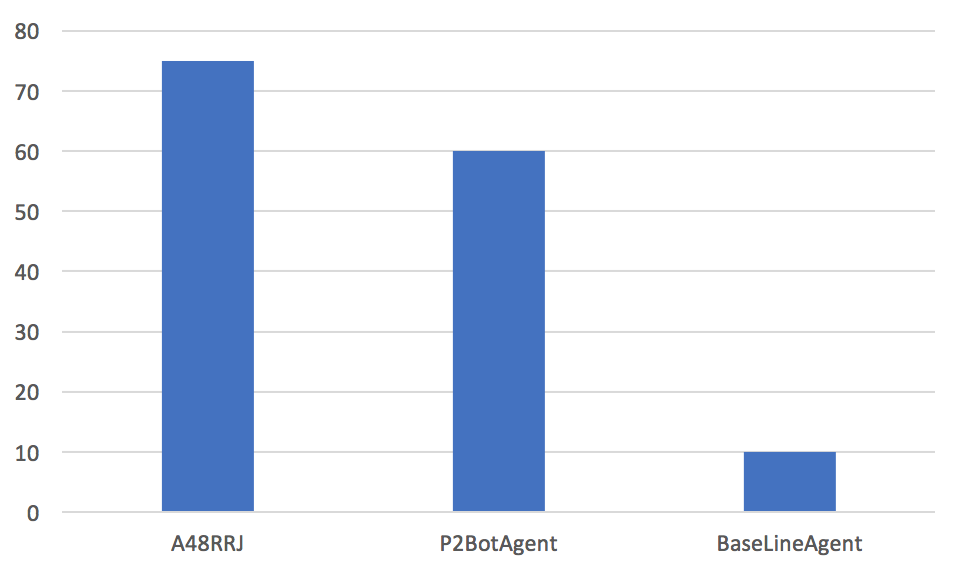
\includegraphics[width=100mm]{nivsup}
        \caption{Total de niveles superados sobre 1000} % Titulo tabla en el indice
        \label{nivsup}

        \center
        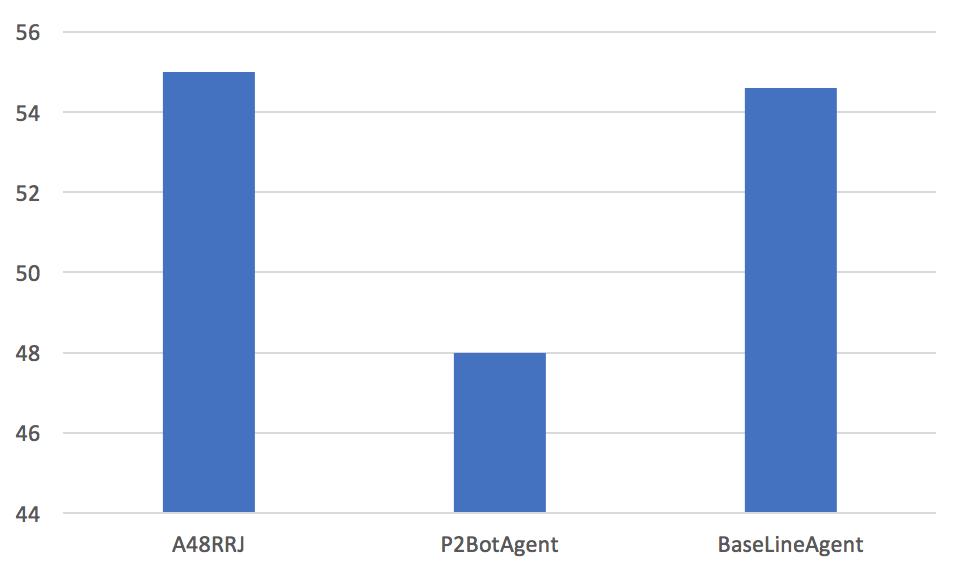
\includegraphics[width=100mm]{porcentaje}
        \caption{ Porcentaje medio de la superación en cada nivel.} % Titulo tabla en el indice
        \label{porcentaje}

        \center
        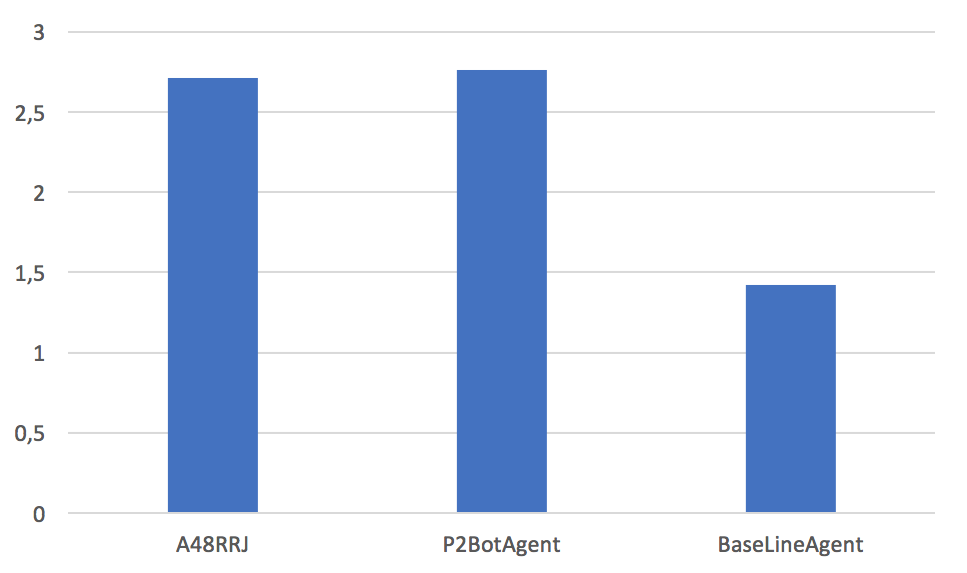
\includegraphics[width=100mm]{nivel}
        \caption{ Media de colisiones con enemigo por nivel.} % Titulo tabla en el indice
        \label{nivel}
    \end{figure}

    \begin{figure}[h!]
        \center
        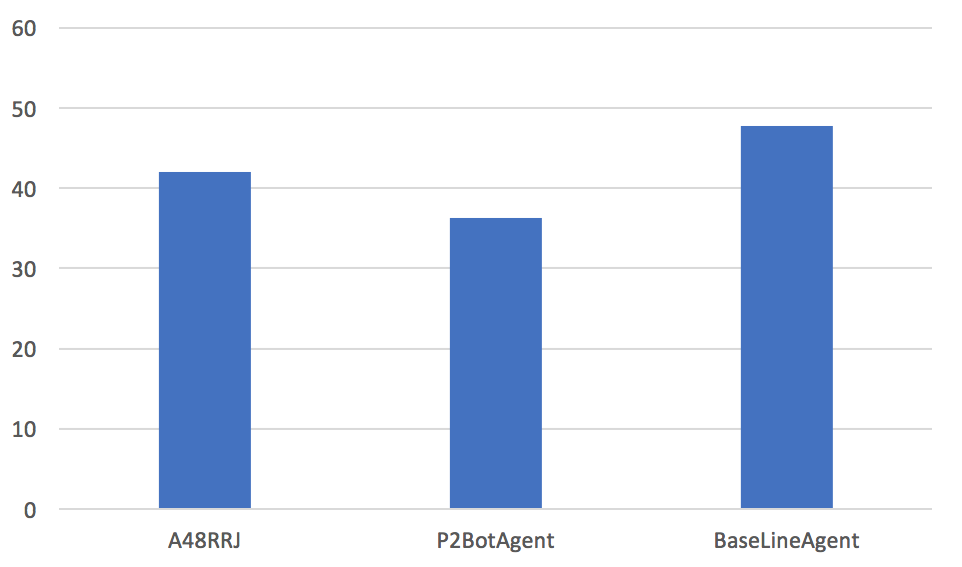
\includegraphics[width=100mm]{monedas}
        \caption{ Media de monedas recogidas por nivel.} % Titulo tabla en el indice
        \label{monedas}
    \end{figure}
    
    
    \begin{figure}[h!]
        \center
        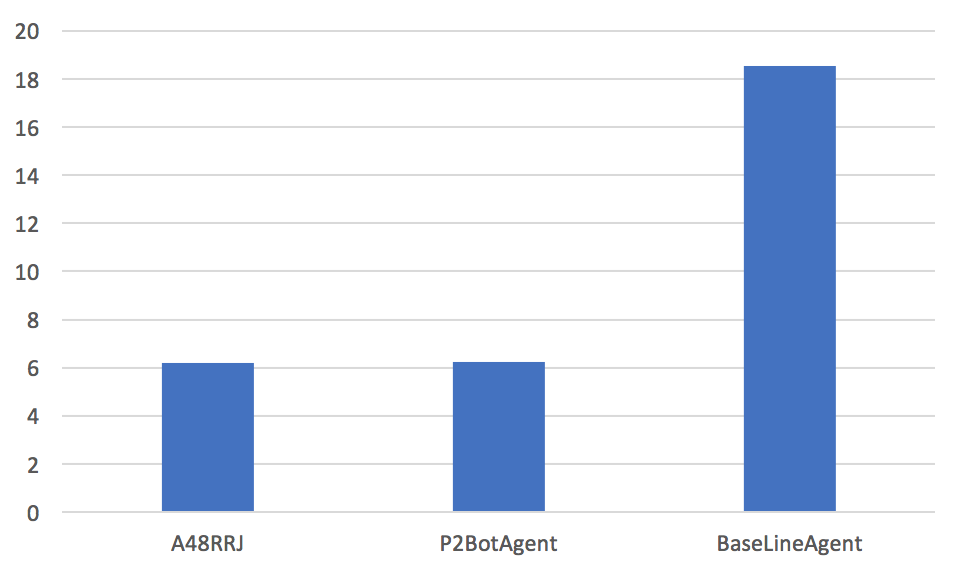
\includegraphics[width=100mm]{muertes}
        \caption{ Media de muertes de enemigos por nivel.} % Titulo tabla en el indice
        \label{muertes}
    \end{figure}
   
    \p{Se ha observado durante la experimentación que con una disposición determinada de pesos, nuestro agente conseguido mediante aprendizaje basado en instancias ha conseguido moverse para atrás para esquivar obstáculos complejos, cosa que el bot A48RRJ no sería capaz de hacer. En la versión entregada no se observan estos comportamientos debido a que se el ajuste de pesos se ha realizado para maximizar la eficiencia del bot. A continuación reflejamos dos de estas situaciones complejas en niveles distintos, donde en verde vemos el camino que realiza mario, y en rojo el que debería hacer para salir de esa situación. }
    \p{\begin{figure}[h!]
        \center
        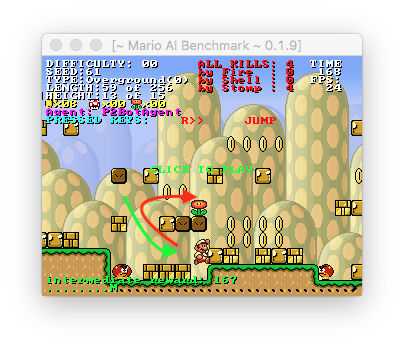
\includegraphics[width=110mm]{61}
        \caption{Nivel 61} % Titulo tabla en el indice
        \label{61}
    \end{figure}
    \begin{figure}[h!]
        \center
        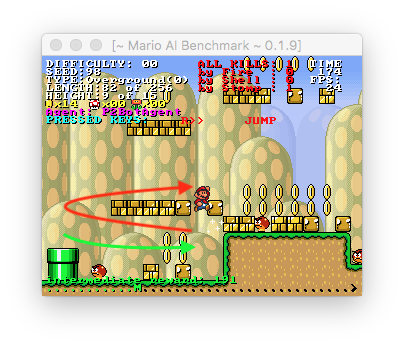
\includegraphics[width=110mm]{98}
        \caption{Nivel 98}
        \label{89}
    \end{figure}}\newpage

    \section{Descripción del material entregado}
\p{Junto a esta memoria, se entrega el siguiente material:}
\begin{itemize}
    \item \textbf{estadísticas.sh:} script en bash utilizado para la captura de estadísticas, estudio y evaluación del agente para pequeños y grandes volúmenes de ejecuciones o niveles. Requiere como dependencia python 3. Su ejecución es la siguiente:
        \begin{center}
            \texttt{./estadísticas.sh\hspace{1em}<agente>\hspace{1em}<num\_niveles>}
        \end{center}
    \item \textbf{weka/ejemplos\_entrenamiento/P2HumanAgent\_1.arff:} fichero que contiene la toma de ejemplos realizada con el agente humano, en formato arff y con cabecera para su tratamiento con weka.
    \item \textbf{weka/ejemplos\_entrenamiento/knowledge\_base.csv:} fichero csv que contiene las instancias de entrenamiento que conforman la base de conocimiento del agente. Es el mismo fichero que P2HumanAgent\_1.arff pero sin cabecera de weka y con nueva extensión.
    \item \textbf{src/ch/idsia/agents/controllers/human/P2HumanAgent.java:} agente humano con el que se ha realizado la toma de ejemplos de entrenamiento contenida en los dos ficheros anteriormente mencionados.
    \item \textbf{src/ch/idsia/agents/controllers/P2BotAgent.java:} agente bot programado con técnicas de inteligencia artificial de aprendizaje basado en instancias. Principal producto de esta práctica. \textbf{Este es el bot programado y no un bot de captura de datos.}
    \item \textbf{src/ch/idsia/tools/TrainingFile.java:} clase java que contiene toda la lógica de captura de ejemplos. Es utilizada por P2HumanAgent.java
    \item \textbf{src/ch/idsia/tools/Instance.java:} clase objeto representación de una instancia, ya sea de entrenamiento o del tick actual del juego. Facilita su tratamiento en el código y su almacenamiento en memoria durante tiempo de ejecución. Es utilizada por P2BotAgent.java
\end{itemize}

\section{Conclusiones}\label{c}
\p{De la realización de un agente inteligente que utiliza técnicas de aprendizaje automático basado en instancias podemos concluir lo siguiente:}
\begin{itemize}
    \item El agente basado en instancias es mucho menos eficiente en términos de recursos computacionales que el agente basado en árboles o reglas de decisión, ya que la revisión de instancias en cada tick añade una carga computacional adicional muy elevada para obtener una decisión a partir de la entrada.

    \item Por el mismo motivo que el punto anterior, el bot de esta práctica (aprendizaje basado en instancias) tendrá un comportamiento más deficiente que el bot de la práctica anterior (árboles/reglas de decisión). Esto es debido a que, en este dominio, necesitamos un comportamiento en tiempo real, por lo que debemos entre otras cosas vigilar el número de instancias de nuestra base de conocimiento, intentando que no sea demasiado elevado. Esto puede suponer una mal resultado en la aplicación de la hipótesis del aprendizaje inductivo, como se ha observado en el apartado anterior \namerefs{e}

    \item Este agente trata mucho mejor (aprende mucho mejor) el comportamiento humano, pues al comparar instancias aisladas en base a criterios objetivos, anula con bastante efectividad la parte aleatoria del comportamiento humano, quedándose solo con los aspectos de aprendizaje importantes, como se indicó en el último apartado de \namerefs{tde}.
\end{itemize}

\section{Comentarios personales}\label{cp}
\p{Si bien la práctica ha sido entretenida y de una dificultad asequible, nos ha costado bastante obtener las situaciones en las que clasificar las instancias, así como determinar los pesos que aplicar a cada atributos en las funciones matemáticas euclídeas.}
\p{Si bien esto es una parte importante de la práctica y algunas decisiones se han tomado en base a criterios objetivos, como se ha detallado en esta memoria o en el código, mucho de estos pesos o clasificaciones se han calculado mediante prueba y error. Por eso, hubiésemos agradecido una guía, una clase, material o algún recurso que nos enseñara cómo calcular estos pesos de forma, si no óptima, al menos más razonada que el típico prueba y error.}
\p{Desarrollar estos apartados de la práctica mediante prueba y error nos ha resultado, además de improductivo y contraproducente (ya que no ha aportado conocimiento reseñable per se), una pérdida elevada de tiempo en un momento del cuatrimestre en el que la carga académica es muy elevada para todas las asignaturas.}

\end{document}